As we have seen in the section \ref{sec:StateOfTheArt}, the current technics which exist nowadays have either higher LDL than the limit established by Council Directive, $100~\becquerel/\liter$, or they are a off-line method (too slow) so those methods cannot be used for tritium monitoring in quasi-real time. 

As a result of these limitations appear the \textit{Tritium} project \cite{TRITIUM}, whose title is "Design, construction and commissioning of automatic stations for quasi-real time monitoring of low radioactive levels of tritium in water".

This project has been funded by Interreg Sudoe program of the EEC in the 2016 call with the reference number SOE1/P4/EO214. The purpose of this project is the development of a tritium monitor in quasi-real time. This monitor consists of a ultra pure water system, which prepare the sample before we introduce it in our detector, the tritium detector where the tritium measure will be done, the active veto and the pasive shielding which reduce the natural background of our tritium detector and several types of electronic which control all these parts of the monitor, analyze the tritium measurement and will send an alarm if the limit of $100~\becquerel/\liter$ is overcome.

The tritium detector is based on measurements of low energy beta radiation from the radioactive decay of tritium. For doing this task this detector consists of scintillator fibers, that we put directly in contact with water which can contain tritium. We need to put both, scintillator fibers and tritium water, in contact due to such a low mean free path of tritium electrons (table \ref{MeanFreePathTritium} of the seccion \ref{sec:TritiumProperties}). Then, the photons produced on this fibers will be read out by several photosensors. The photosensors which we have tested in this experiment are photoelectron multiplier tubes (PMT) and silicon photoelectron multiplier (SiPM) arrays. 

The difficulty when we try to measure tritium is to distinguish these signals from the background. This is because tritium signals are small since tritium events has low energy ($\sim~\keV$) and this is the energy range in the spectrum where there are more background counts (the lower energy, the more background events). We will use coincidence techniques in order to reduce the counts from the background.

It is important to check the water tightness of each prototype because if the water reaches the photosensor it will be irreparably damaged. On top of that if we use high concentrations of tritium in water for laboratory tests we can contaminate this laboratory, which could be dangerous for the healthy of the workers and it could spoil measurements of future experiments.

Finally this monitor will be installed in the Arrocampo dam, Almaraz, Spain, where the Almaraz nuclear power plant release the water which is used in their cooling system, Figure \ref{fig:Arrocampo}. This NPP has two nuclear reactors whose type is PWR. This dam is located near the Tajus river, which is the largest river in Spain, $1007~\kilo\meter$. This river cross from Aragon (Spain) to Lisbon (Portugal) and flows into the atlantic ocean. This river is used for an important quantity of animals, plants and even humans because the water of this river is used as drinking water by the spanish and portuguese people. Therefore the international cooperation in order to maintain the quality of this water is very important.

\begin{figure}[hbtp]
 \centering
  \subfloat[Arrocampo dam and Almaraz Nuclear Power Plant]{
   \label{fig:Arrocampo_Dam}
    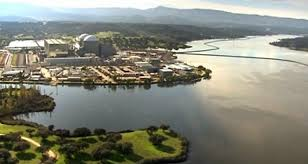
\includegraphics[width=0.47\textwidth]{2Introduction/ArrocampoDam.jpeg}}
  \subfloat[Tajus river along Spain and Portugal]{
   \label{fig:TajusRiver}
    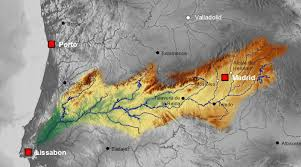
\includegraphics[width=0.53\textwidth]{2Introduction/RioTajo.jpeg}}
 \caption{Arrocampo dam, Almaraz NPP and Tajus river}
 \label{fig:Arrocampo}
\end{figure}

The \textit{Tritium} collaboration is a international group consisting of a consortium of 6 different southwestern european institution of 3 different countries: The University of Aveiro, in Portugal, The University of Bordeaux and the CNRS  (Section Aquitaine-Limousin), in France and the University of Extremadura, \textit{Junta de Extremadura} and University of Valencia, in Spain.

FOTOO TRITIUM

Each institution has focused in the development of a different part of all this project:
\begin{itemize}
\item{} First, the Extremadura group has developed and installed the ultra pure water system with wich we get water with very low conductivity, $\sigma \approx 10 ~\mu S / \cm$. The conductivity of the water before the cleaning proces is around $ 1000 ~\mu S / \cm$. This clean process is very important for two reasons. On the one hand, it is important for maintaining our detector very clean, which is a critical point. On the other hand, it's important because with this process we reduce the natural background since we remove several natural radiactive isotopes that there are in this water (except tritium) such as $\ce{^{222}Rn}$, $\ce{^{40}K}$ or $\ce{^{137}Cs}$. This system will be explained in the chapter \ref{chap:Ultrapure}.

\item{} Second, french group has develop the pasive shielding where our detector will work inside. It is based in ultra radiopure lead with very low intrinsic activity. The objective of this pasive shielding is to reduce the external natural background that affect to our system, for this reason we use lead. Obviously, this shielding doesn't have to affect to the measurement of our system, for this reason we use radiopure elements with very low intrinsic activity. This shielding will be explained in the chapter \ref{chap:Shields}, section \ref{sec:PasiveShields}.

\item{} Third, The Portugal and Spanish people has developed the simulations about this system. The program which we have used in this project is GEANT 4, which is a simulation package. It consiste in a extensive C++ library with which we can design the geometry of our detector, the physical processes which happen there, etc. This simulation will be explained in the chapter \ref{chap:Simulations}.

\item{} Lastly, The Portugal and Spain people has collaborated for designing, developing and building four different prototypes of tritium detector and active vetos for removing cosmic events. These prototypes and vetos will be explained in the chapter \ref{chap:Prototypes}.

\end{itemize}

The tritium level which we want to mesure follow the ALARA principle (As Low As Possible Achievable) and to get it there are important characteristics which our tritium detector must have:

\begin{itemize}

\item{} \textit{Compact}. This is important because in the place where this detector will be installed the useful space that we can use is finite.

\item{} \textit{Thin active volume and large active area}. On the one hand, we have to take into account that, as we have seen in the table \ref{MeanFreePathTritium} of the seccion \ref{sec:TritiumProperties}, the mean free path of the $\beta$ particle of tritium decay is very low so we need to work with thin active volumes. In the practice, Active thickness beyond the mean free path of the tritium will only contribute to the background. On the other hand, as we have checked in the seccion \ref{sec:StateOfTheArt} the efficiency of this type of detector scales with the active area so we need to design our detector with the largest possible active area.

\item{} \textit{High sensitivity to tritium}. We are going to work with low tritium activities so we need to reduce as much as possible the non-detected tritium events.

\item{} \textit{High specificity to tritium}. We need that our detector is able to distinguish the tritium signal of the signal of other radiactive elements which can be present in the initial sample.

\item{} \textit{Quasi-real time response}. As we have seen it is important that our sistem can work in quasi-real time in order to detect any problem as fast as possible. 

\item{} \textit{Rugged system}. Finally, we have to take into account that our objective will be installing an automatical system which will work during a lot of years without specialized people so we need that our monitor are rugged. 

\end{itemize}

In order to get the measurement in quasi-real time we need to work \textit{in situ}, that's, we need that our detector is able to work in the same place that we take the sample. Whit the work \textit{in site} we achieve:

\begin{itemize}
\item{} a faster monitor because we eliminates the process of taking the sample, the chain-of-custody until this sample arrive to this laboratory and the complexity which involve these tasks. 

\item{} a better monitor since if we can work \textit{in site}, our measurements can be more frequent hence we will can identify cahnges in the activity earlier.

\item{} a cheaper monitor because we have not only the material costs attached to the sample collection, chain-of-custody of this sample, shipping of this sample to the laboratory, etc. but we have also eliminated the costs attached to the specialized staff who are involving in these tasks. Our detector will only need frequent calibrations each time in order to ensure its correct operation.

\item{} a safer monitor since the personal exposure dose is reduced and the changes in activity are detected fastly. On top of that we remove the possibles mistakes which can be done by specialized staff.

\end{itemize} 